\subsection{Implementación mediante celdas enlazadas}
Esta implementación es muy parecida a la implementación mediante celdas enlazadas en árboles binarios, la única diferencia es que en la parte privada no almacenamos hijos derechos, si no que almacenamos hermanos derechos, ya que en nuestro TAD, el concepto de hijo derecho ya no tiene sentido.

\begin{figure}[h]
  \begin{center}
    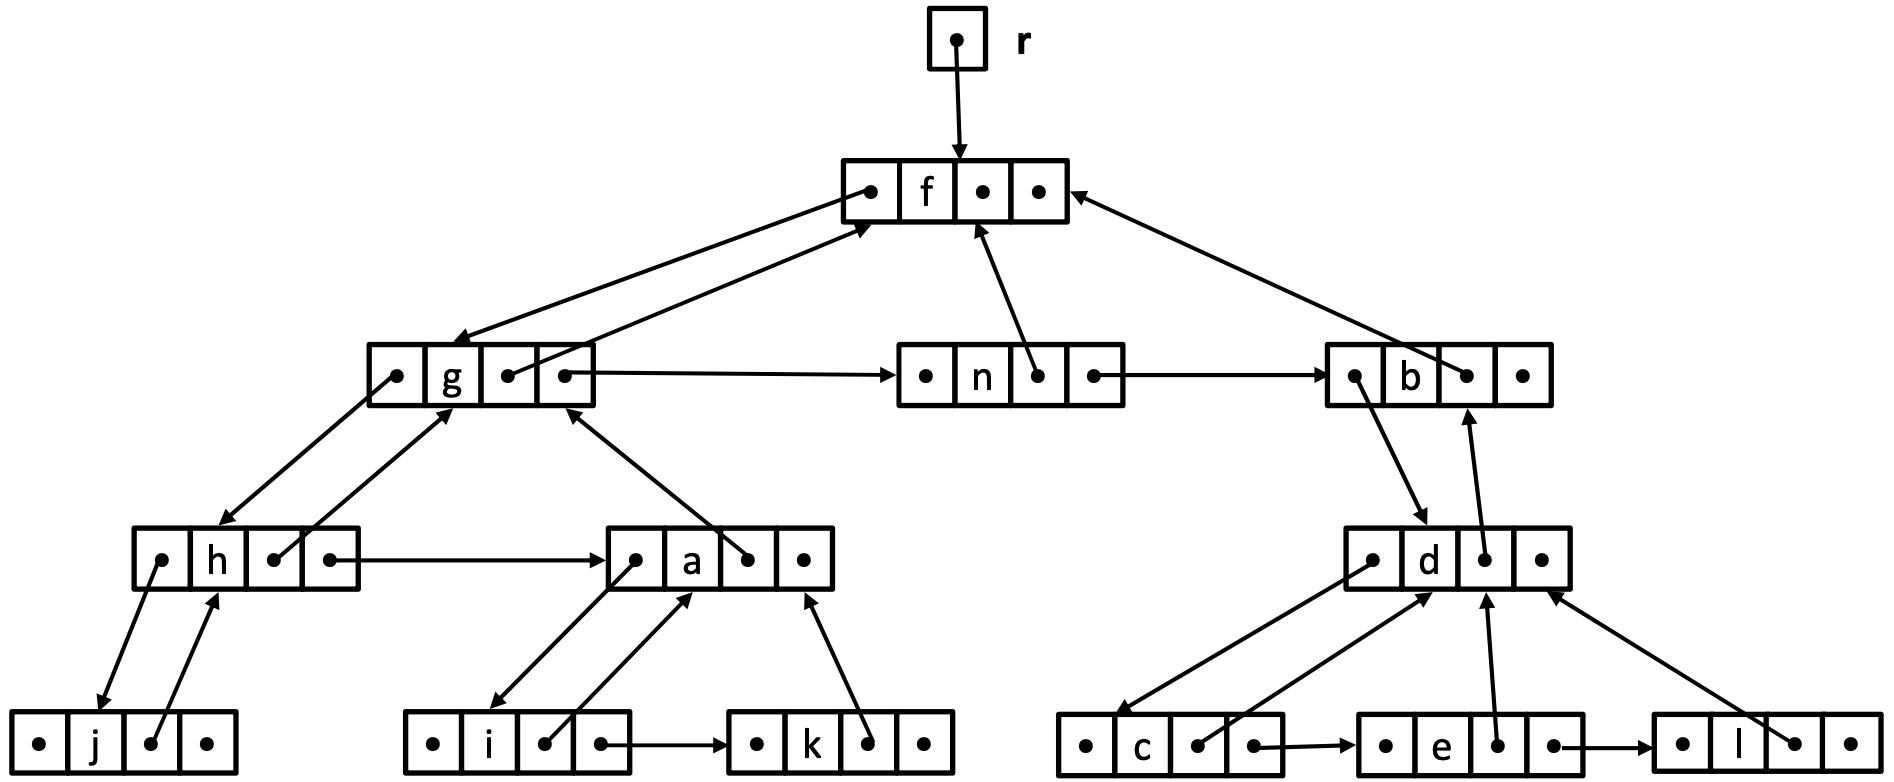
\includegraphics[width=.7\textwidth]{assets/AgenEnla.png}
  \end{center}
  \caption{Representación de la implementación mediante celdas enlazadas}
\end{figure}

Por tanto, la parte privada del TAD nos quedaría:
\begin{verbatim}
template <typename T> class Agen{
  public:
    //Métodos vistos en la especificación del TAD
  private:
    struct celda{
      T elto;
      nodo padre,hizq,heder;
      celda(const T& e, nodo p = NODO_NULO):elto(e),padre(p),
        hizq(NODO_NULO),heder(NODO_NULO){}
    };
    nodo r; //nodo raíz del árbol
};
\end{verbatim}

